
\section*{Zadanie 10.}
\begin{task}
Wymienić najczęściej stosowane w praktyce rodzaje linii TEM. Narysować (w przekrojach wzdłużnym i poprzecznym) rozkłady pól $E$ i $H$ dla rozchodzącej się w nich fali bieżącej. Podać cechy każdego z wymienionych typów linii determinujące ich zakres zastosowań praktycznych.\\
\end{task}

\begin{solution}
\begin{itemize}
\item Najczęściej stosowane linie TEM:
	\begin{itemize}
	\item linia współosiowa (najczęściej)
	\item symteryczna linia paskowa
	\item niesymetryczna linia paskowa (linia mikropaskowa, quasi-TEM)
	\item symetryczna linia dwuprzewodowa
	\end{itemize}
\item linia współosiowa - rozkład pól\\
$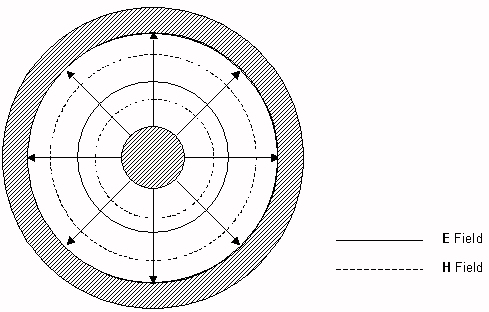
\includegraphics[scale=1.5]{10_1}$    $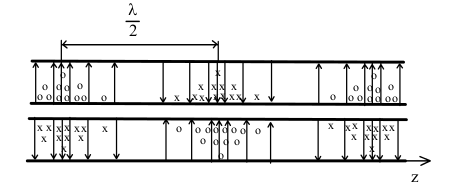
\includegraphics[scale=0.7]{10_2}$
\item symetryczna linia paskowa - rozkład pól\\
$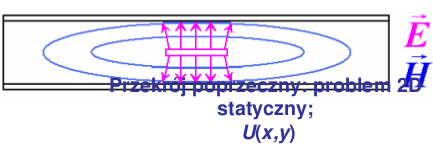
\includegraphics[scale=0.7]{22_2}$    $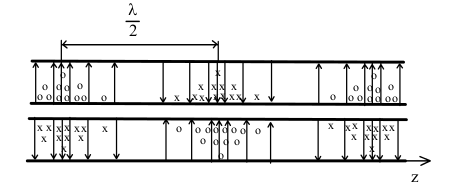
\includegraphics[scale=0.6]{10_2}$
\item niesymetryczna linia paskowa - rozkład pól\\
$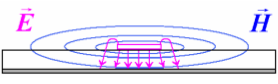
\includegraphics[scale=1]{10_3}$    $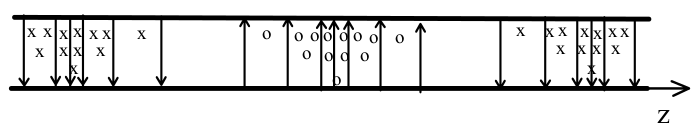
\includegraphics[scale=0.6]{35_2}$
\item Symetryczna linia dwuprzewodowa - rozkład pól\\
$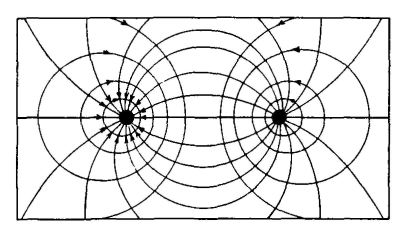
\includegraphics[scale=0.6]{10_4}$
\item Cechy linii współosiowej:
	\begin{itemize}
	\item dobre ekranowanie od pól zewnętrznych (na zewnątrz linie pola elektromagnetycznego są zerowe)
	\item ograniczony zakres impedancji charakterystycznych $Z_{c}=\cfrac{Z}{2\pi}\ln{\cfrac{a}{b}}$
	\item trudno robić rozgałęzienia oraz odcinki linii sprzężonych
	\item trudności z dołączaniem elementów skupionych
\end{itemize}
Typowe zakresy częstotliwości: kilkadziesiąt $MHz$ do kilku $GHz$. Czasami stosowana do niskich częstotliwości. Wynika to z faktu, że pola przesyłanej fali dla tej linii są dobrze odizolowane od pól zewnętrznych, a więc fala ta nie jest zakłócana z zewnątrz ani też nie zakłóca innych fal.

\item Cechy linii symetrycznej paskowej:\\ W stosunku do linii współosiowej znaacznie ułatwia budowanie rozgałęzień i linii sprzężonych. Stosowana do między innymi budowy filtów i sprzęgaczy mikrofalowych.\\
Przy odpowiednio szerokich płytach ekranujących (górnej i dolnej o jednakowym potencjale) możemy uznać, że pole, podobnie jak w linii współosiowej jest zamknięte wewnątrz linii, a więc dobrze odizolowane od otoczenia.

\item Cechy linii niesymetrycznej paskowej:
	\begin{itemize}
	\item łatwość w montowaniu elementów skupionych
	\item łatwośći przystosowania do masowej produkcji
	\item zależności długości fali od szerokości linii
	\item zależność parametrów od częstotliwości (dyspersja)
	\item gorsze odseparowanie od pól zewnętrznych oraz promieniowanie
	\end{itemize}
Zastosowanie: Powszechnie stosowana w układach analogowych, układach cyfrowych oraz układach scalonych
\item Cechy linii symetrycznej dwuprzewodowej:
	\begin{itemize}
	\item stosowana w energetyce
	\item stosowana do wysokich częstotliwości
	\item rozpraszanie pola na zewnątrz, sygnał przesyłany może sprzęgać się z innymi sygnałami
	\item prostota budowy
	\item możliwość realizacji linii o dużej impedancji charakterystycznej (rzędy kilkuset $\Omega$ )
	\item stosowana do połączenia odbiorników telewizyjnych z antenami
	\end{itemize}
\end{itemize}
\end{solution}